% GP intro

\begin{frame}
	\frametitle{Gaussian Processes}
	\begin{figure}[tbh]
		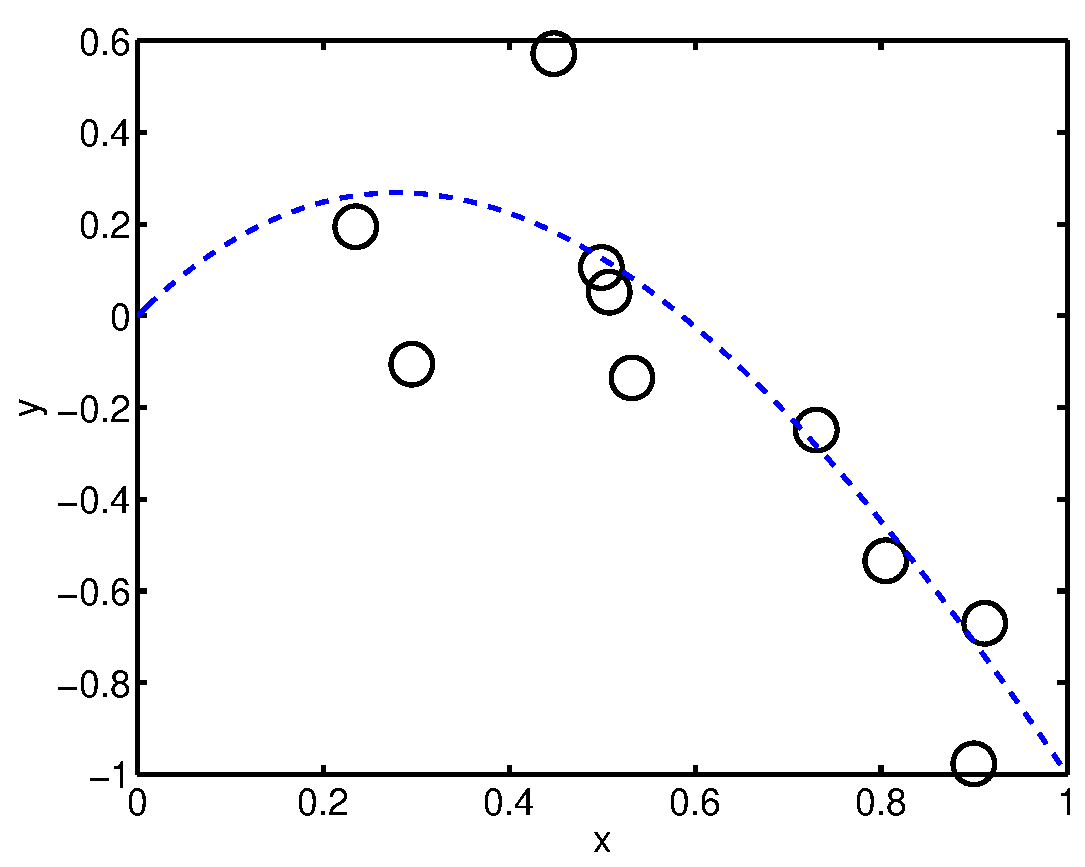
\includegraphics[width=0.7\linewidth]{gpintro_data.pdf}		
		\centering\caption{\label{fig:gpintro_data}A familiar problem: learn the underlying function (blue) from the observed data (crosses).}
	\end{figure}
\end{frame}

\begin{frame}
	\frametitle{A parametric approach?}
	\begin{figure}[tbh]
		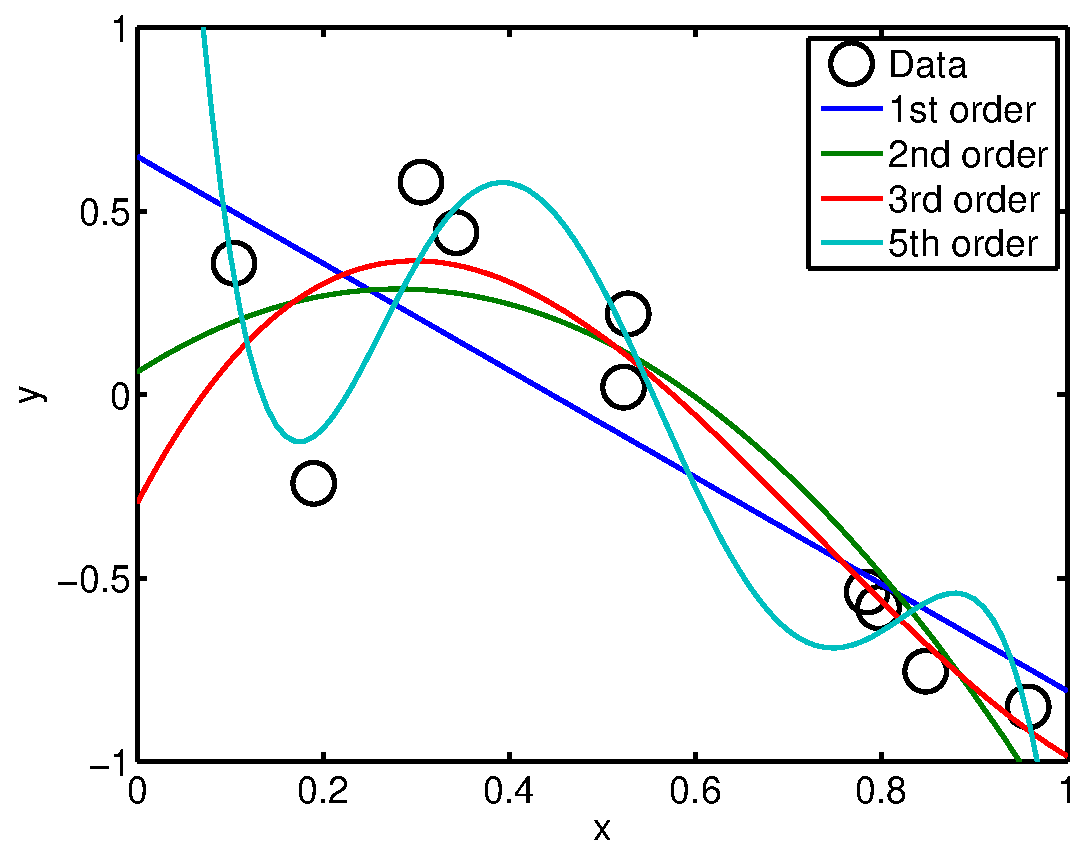
\includegraphics[width=0.7\linewidth]{gpintro_poly.pdf}		
		\centering\caption{\label{fig:gpintro_poly}Polynomials fitted by least squares.}
		It's easy to under and over-fit. What if we have no idea of the parametric form of the function?
	\end{figure}
\end{frame}

\begin{frame}
	\frametitle{A non-parametric approach - Gaussian Processes}
	\begin{itemize}
		\item Rather than forcing us to choose a particular parametric form, a \ac{GP} allows us to place a prior distribution directly on \emph{functions}
		\item With a \ac{GP} prior we can:
		\begin{itemize}
			\item Sample functions from the prior
			\item Incorporate data to get a \emph{posterior} distribution over functions
			\item Make predictions
		\end{itemize}
	\end{itemize}
\end{frame}

\begin{frame}
	\frametitle{Visual example -- prior}
	\begin{figure}[tbh]
		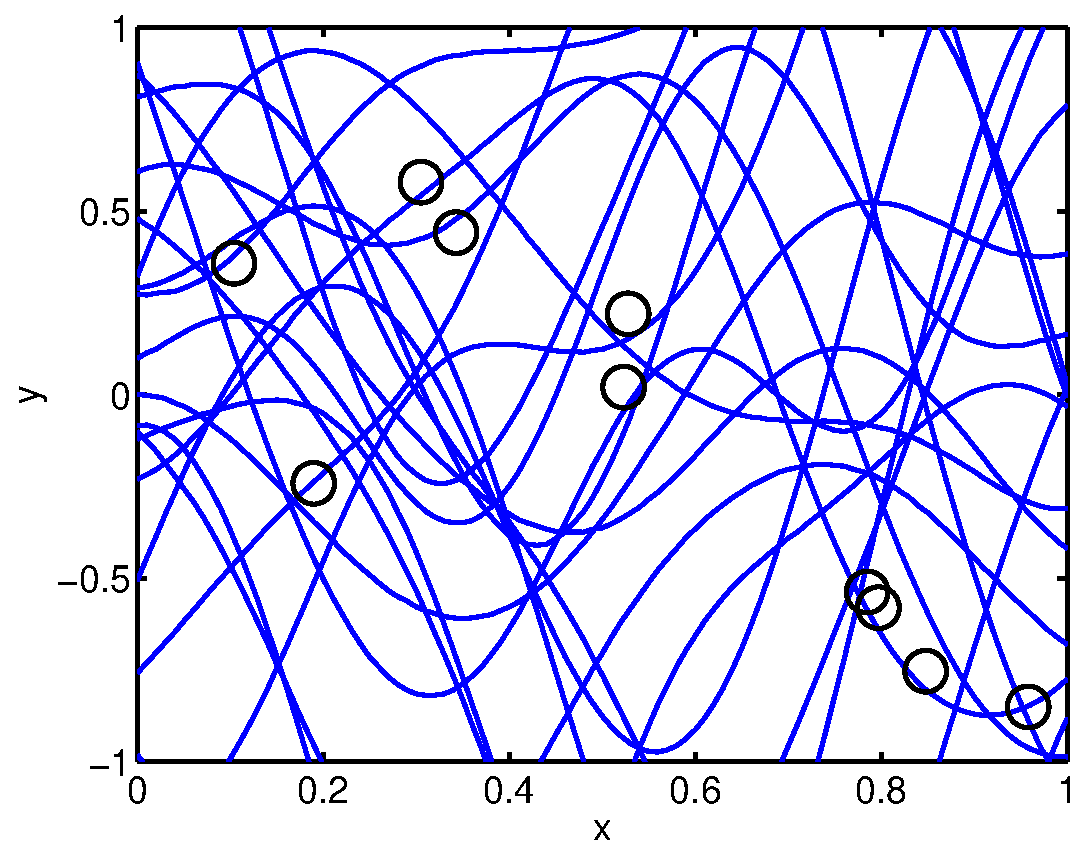
\includegraphics[width=0.7\linewidth]{gpintro_prior.pdf}		
		\centering\caption{\label{fig:gpintro_prior}Some functions drawn from a \ac{GP} prior.}
	\end{figure}
\end{frame}

\begin{frame}
	\frametitle{Visual exmample -- posterior}
	\begin{figure}[tbh]
		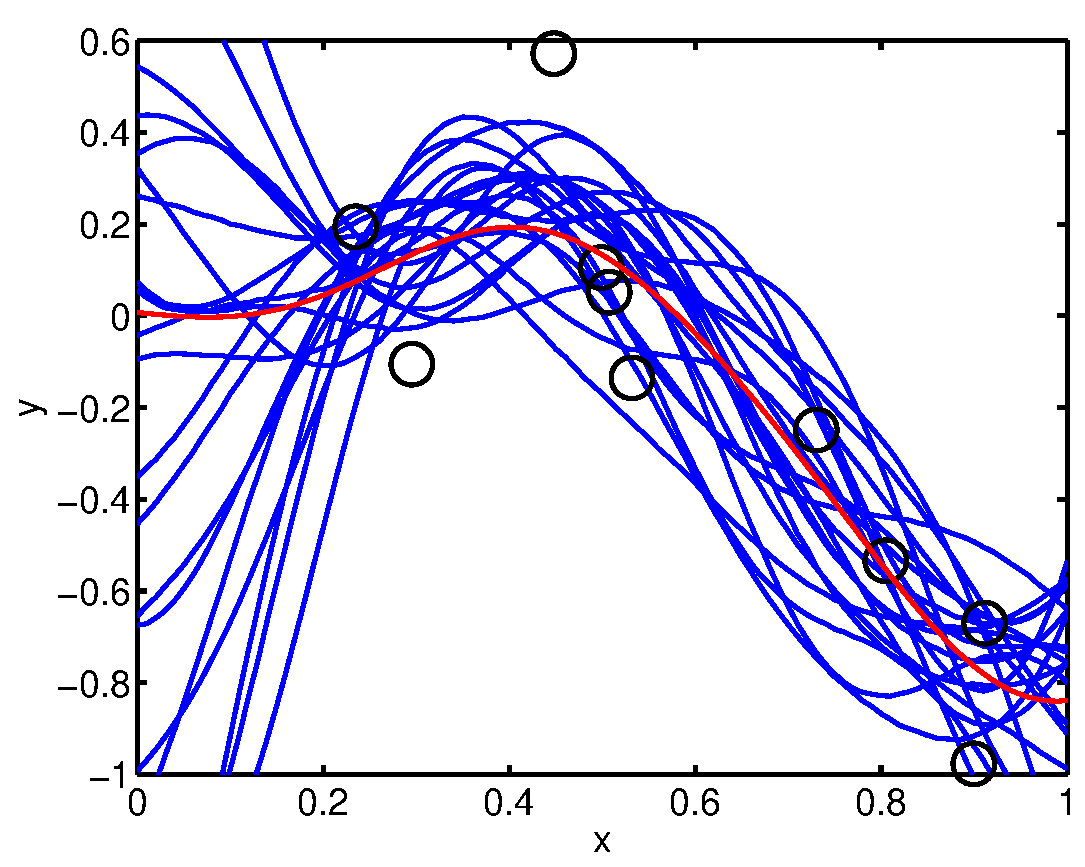
\includegraphics[width=0.7\linewidth]{gpintro_posterior.pdf}		
		\centering\caption{\label{fig:gpintro_posterior}Some functions drawn from the \ac{GP} posterior. Posterior mean is shown in red.}
	\end{figure}
\end{frame}

\begin{frame}
	\frametitle{Visual example -- predictions}
	\begin{figure}[tbh]
		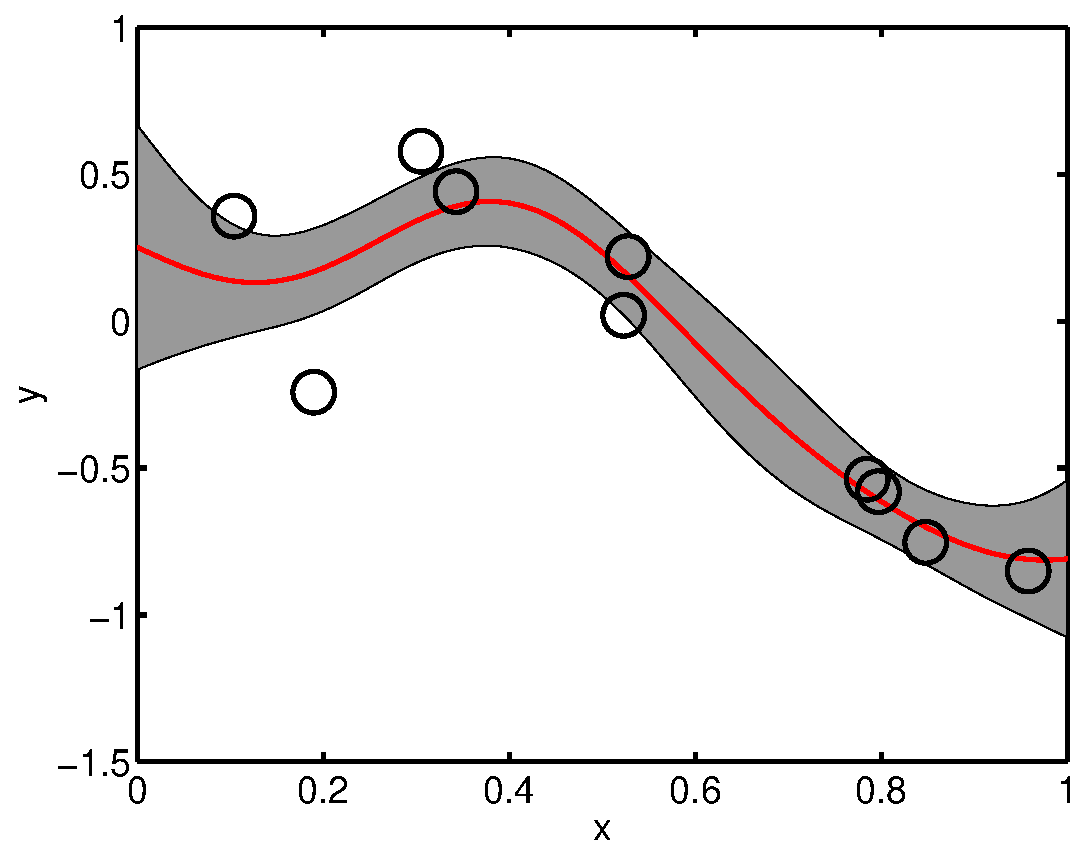
\includegraphics[width=0.7\linewidth]{gpintro_predictions.pdf}		
		\centering\caption{\label{fig:gpintro_predictions.pdf}Predictive mean and standard deviations.}
	\end{figure}
\end{frame}

\begin{frame}
	\frametitle{Some formalities}
	\begin{itemize}
		\item We observe $N$ training points, each of which consists of a set of features $\bx_n$ and a target $y_n$.
		\item We can stack all of the $y_n$ into a vector and $\bx_n$ into a matrix:
		\[
		\by = \left[
			\begin{array}{c}
			y_1 \\ y_2 \\ \vdots \\ y_N
			\end{array}
		\right],~~~
		\bX = \left[
		\begin{array}{c}
			\bx_1^T \\ \bx_2^T \\ \vdots \\ \bx_N^T
		\end{array}
		\right]
		\]
	\end{itemize}

\end{frame}

\begin{frame}
	\frametitle{GP definition}
	\begin{itemize}
		\item The GP assumes that the vector of \emph{all possible} $y_n$ is a draw from a \ac{MVG}.
		\item We don't observe \emph{all possible} values (if we did, we wouldn't need to make predictions!)
		\visible<2->{\item But the marginal densities of a \ac{MVG} are also \ac{MVG}s so the subset we observe are also a draw from a \ac{MVG}.
		\[
			\by \sim {\cal N}(\boldsymbol\mu,\mathbf{C})
		\]}
		\visible<3->{\item With mean $\boldsymbol\mu$ (normally 0) and covariance $\mathbf{C}$} 
		\visible<4->{\item $\bx_n$ looks to have disappeared -- we find it inside $\mathbf{C}$}
	\end{itemize}
\end{frame}

\begin{frame}
	\frametitle{GP definition}
	\begin{figure}[tbh]
		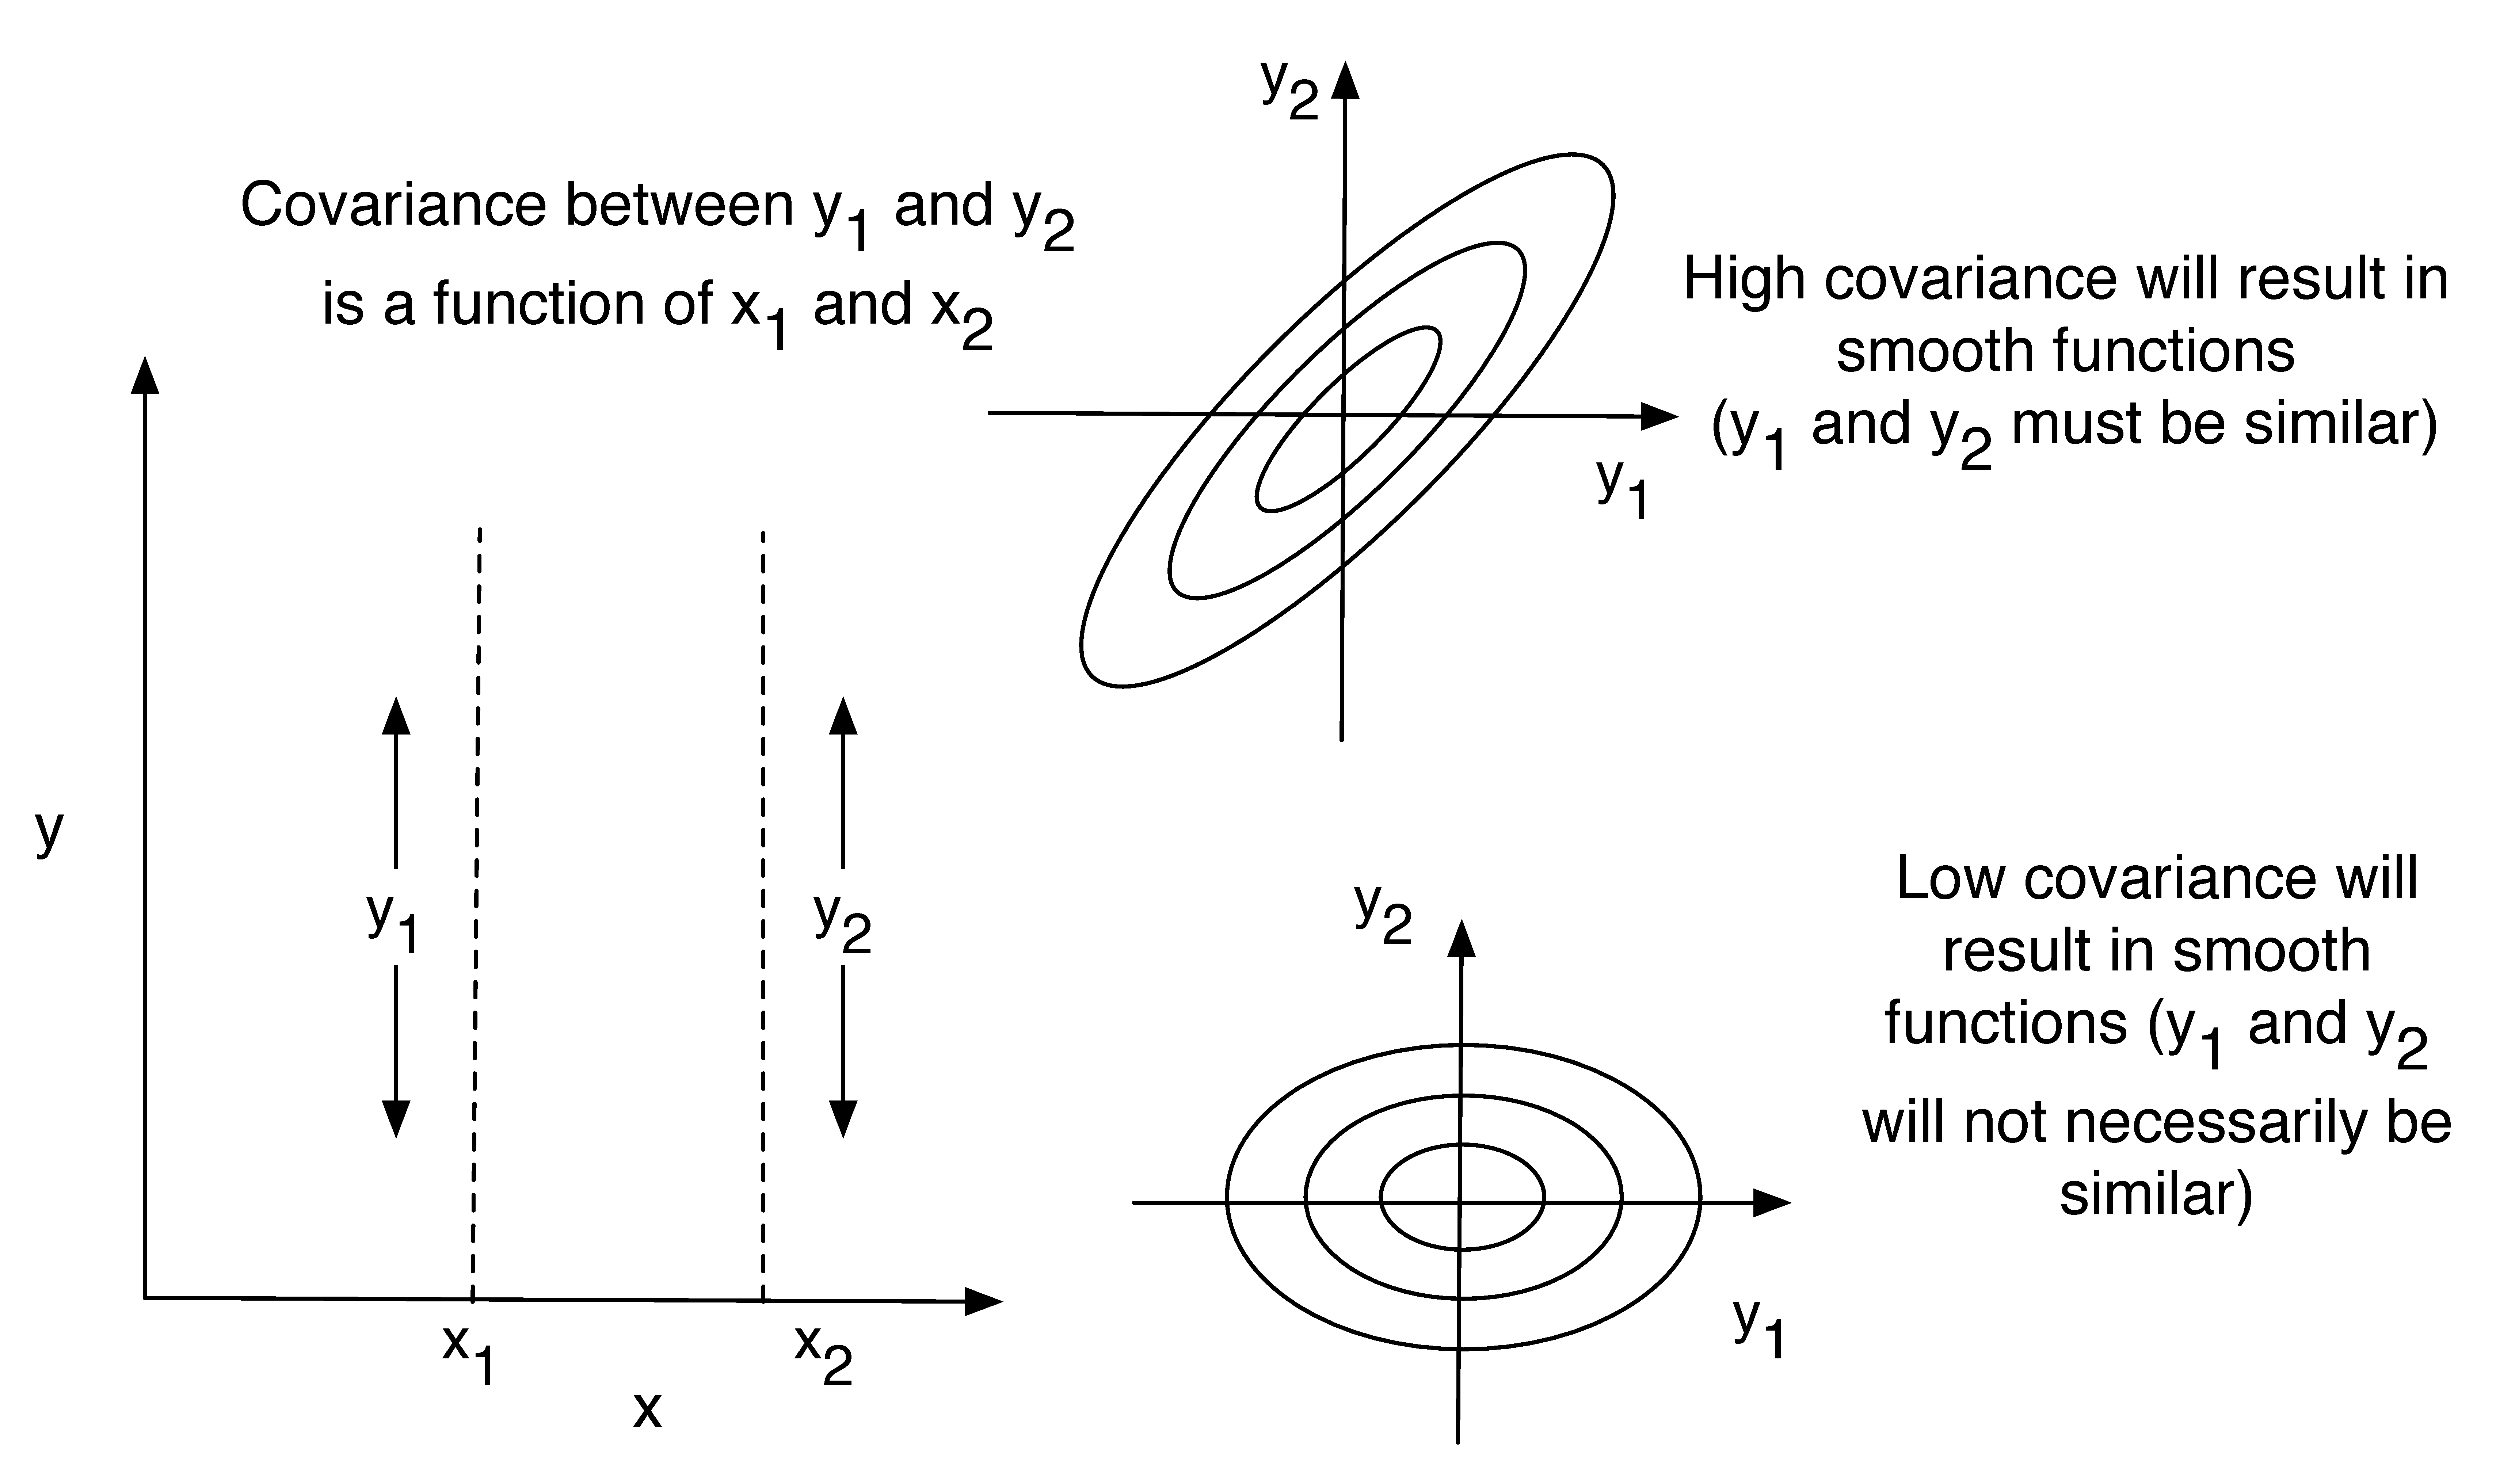
\includegraphics[width=\linewidth]{GPcartoon.pdf}		
		\centering\caption{\label{fig:GPcartoon}Schematic of GP prior for two function values.}
	\end{figure}
\end{frame}


\begin{frame}
	\frametitle{Covariance functions}
	\begin{itemize}
		\item By choosing a covariance function, we are making an assumption on the \emph{smoothness} of the regression function.
		\item Common choices:
		\begin{itemize}
			\item Linear: $C(\bx_1,\bx_2) = \bx_1^T\bx_2$
			\item RBF: $C(\bx_1,\bx_2) = \exp\left\{-0.5\gamma ||\bx_1 - \bx_2||^2 \right\}$
			\item And many, many more.
		\end{itemize}
		\item More details: \url{http://www.gaussianprocess.org/gpml/}
		\begin{itemize}
			\item (Free) book
			\item Code
		\end{itemize}
	\end{itemize}
\end{frame}

\begin{frame}
	\frametitle{Hyper-parameters}
	\[
C(\bx_1,\bx_2) = \exp\left\{-0.5\gamma ||\bx_1 - \bx_2||^2 \right\}
	\]
	\begin{figure}[tbh]
		\subfigure[$\gamma=1$]{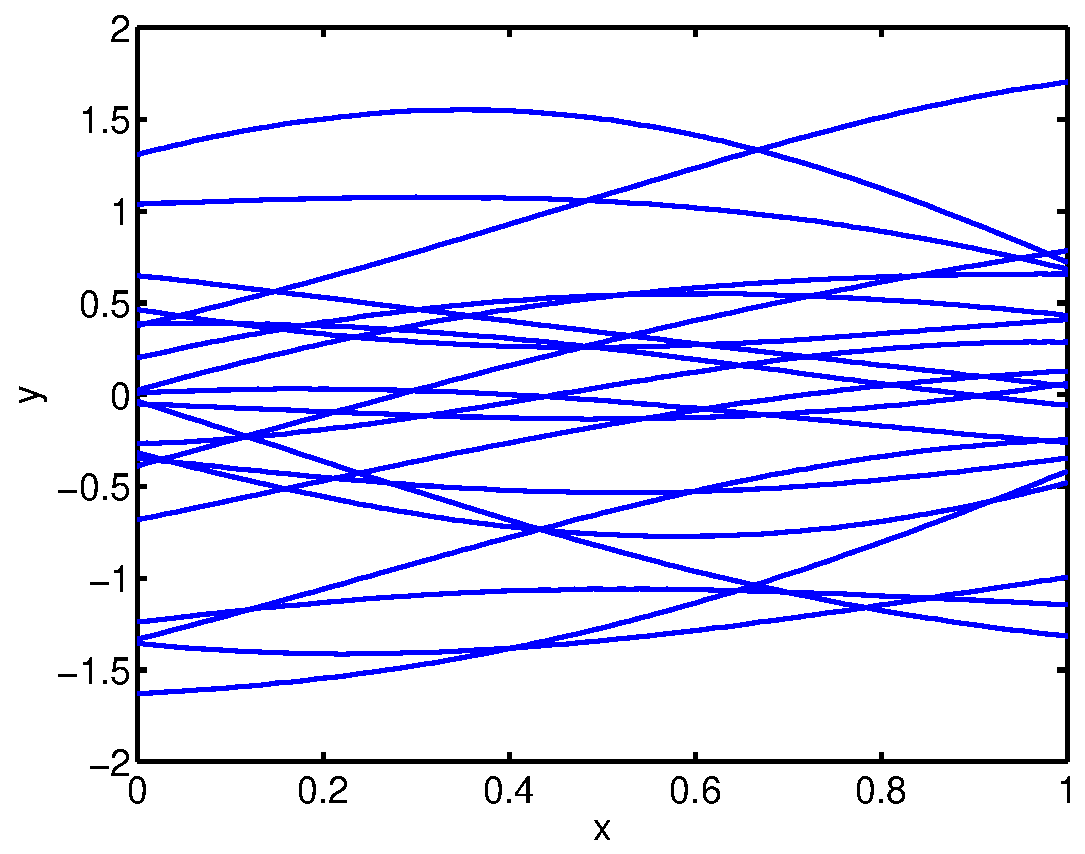
\includegraphics[width=0.32\linewidth]{gpintro_prior_hyp1.pdf}}
		\subfigure[$\gamma=10$]{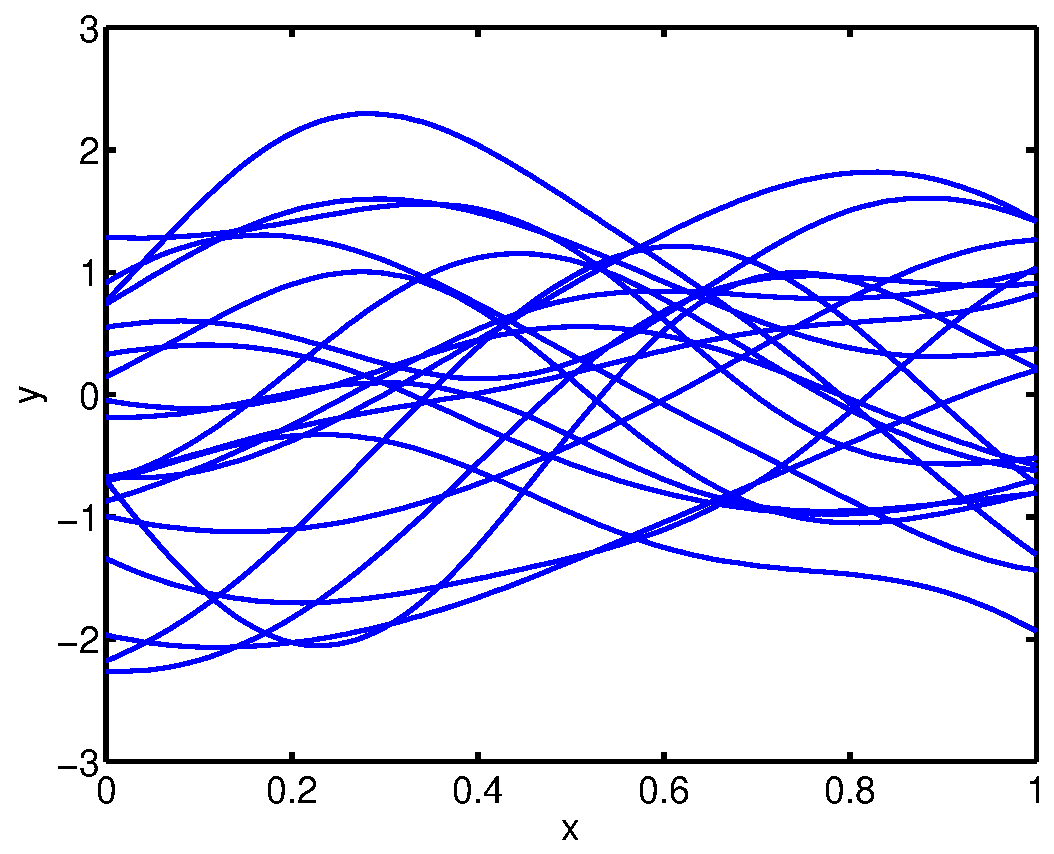
\includegraphics[width=0.32\linewidth]{gpintro_prior_hyp10.pdf}}
		\subfigure[$\gamma=100$]{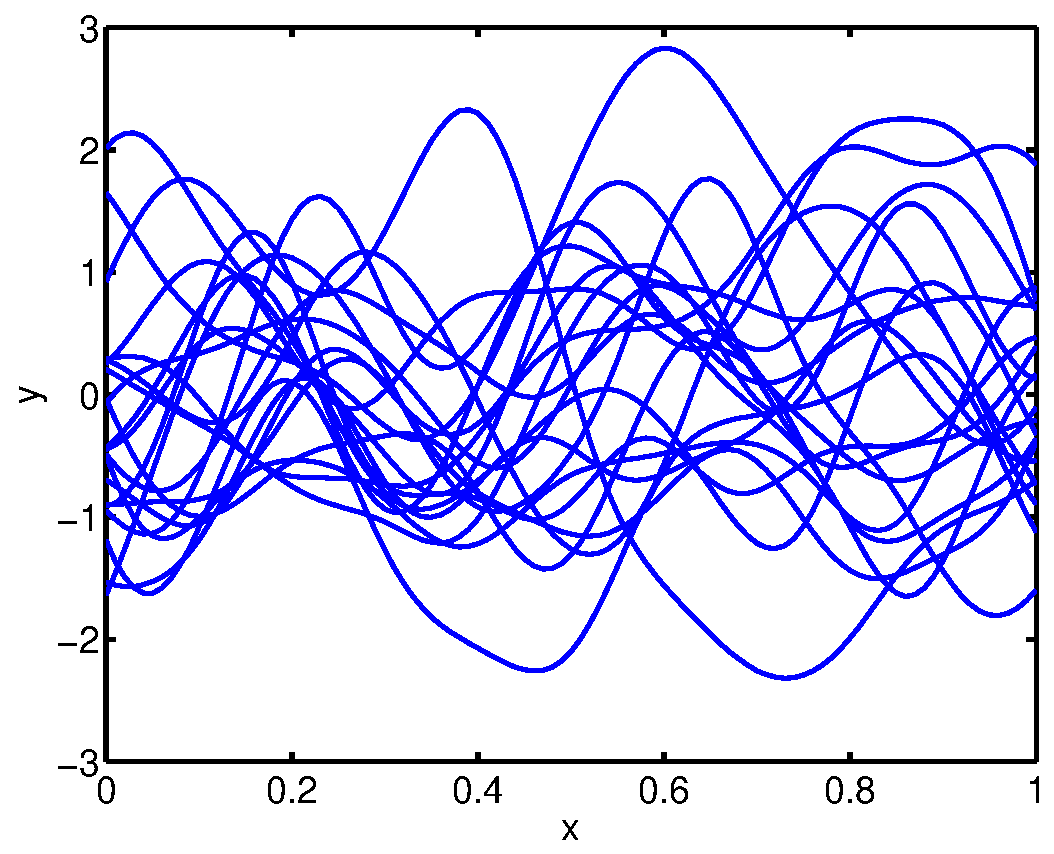
\includegraphics[width=0.32\linewidth]{gpintro_prior_hyp100.pdf}}
		\centering\caption{\label{fig:hyper}Varying hyper-parameters in an RBF covariance varies the smoothness of the function.}
	\end{figure}
\end{frame}

\begin{frame}
	\frametitle{Optimising hyper-parameters}
	
\end{frame}

\begin{frame}
	\frametitle{Making predictions}
	
\end{frame}

\begin{frame}
	\frametitle{GP classification}
	
\end{frame}